\chapter{Implementación}

Neste capítulo se comentarán os aspectos máis relevantes da implementación da nosa plataforma, ben sexa polo uso de librerías externas ou porque requiriron un desenvolvemento especial. Farase mención a detalles do servidor, da aplicación Android así como da autenticación a través de Google.


\section{Servidor}
Nesta sección vanse tratar todos os detalles de implementación propios do servidor, dende o acceso á base de datos ata a construción dos servizos web. En todo o servidor utilizouse a ferramenta de Spring para configurar a transaccionalidade, a inxección de dependencias ou a creación dos servizos web.

A autenticación con Google terá a súa propia sección ao final do capítulo.


\subsection{Acceso á base de datos}
Para o acceso á base de datos utilizouse directamente JDBC sen facer uso de ningunha ferramenta de mapeo obxecto-relacional como pode ser Hibernate. Escolleuse esta opción por ser un sistema sen moita complexidade á hora de gardar ou eliminar rexistros en base de datos e cun número de táboas non moi alto. En sistemas pequenos non se aproveitan os beneficios que poden ter estas ferramentas e desta maneira afórrase a súa configuración.

\begin{figure}[tbh] 
	\begin{center}
		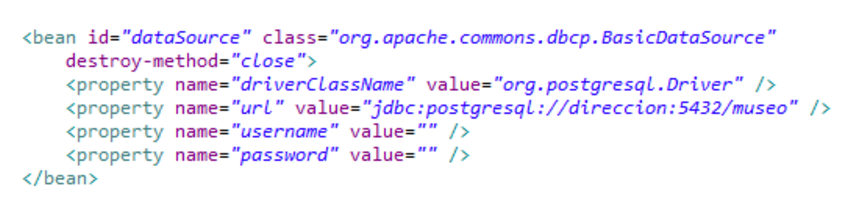
\includegraphics[width=0.85\textwidth]{figures/codigo/configuracionBD}
		\caption{Configuración da base de datos no ficheiro XML.}
		\label{fig:configuracionBD}
	\end{center}
\end{figure}

Na figura~\ref{fig:configuracionBD} pódese observar a configuración do data source que permite a conexión coa BD no servidor. Nel indícase o nome do driver utilizado para a conexión, así como a URL onde se atopa a base de datos. Tamén é preciso engadir o nome de usuario e o contrasinal que permiten o acceso.

Na mesma figura tamén se observa a definición do bean NamedParameterJdbcTemplate, que permite a escritura de consultas con parámetros utilizando nomes, e que se sirve do data source para lograr a conexión coa base de datos. As consultas utilizadas pola plantilla de JDBC sitúanse no ficheiro queries.properties, onde Spring as localiza para despois inxectalas directamente nos DAOs.

\begin{figure}[tbh] 
	\begin{center}
		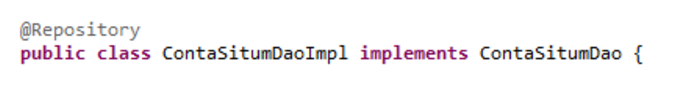
\includegraphics[width=0.65\textwidth]{figures/codigo/dao}
		\caption{Clase de implementación dun DAO.}
		\label{fig:dao}
	\end{center}
\end{figure}

Creouse unha implementación para cada un dos DAOs amosados na sección de deseño. Dentro deles fanse todas as accións permitidas sobre as táboas que representa cada VO. A implementación de cada un dos DAOs segue a mesma estrutura. Para indicarlle a Spring que estas son as clases que se utilizan para a recuperación de información da base de datos etiquétanse con \emph{@Repository}, e dese xeito poder inxectalas na capa de xestión da información (manager). Esta etiqueta pódese ver na figura~\ref{fig:dao}.

\begin{figure}[tbh] 
	\begin{center}
		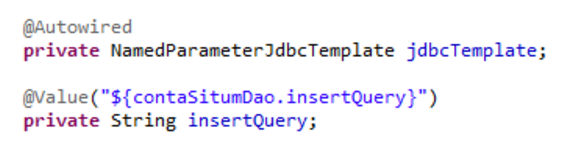
\includegraphics[width=0.5\textwidth]{figures/codigo/inxeccionDao}
		\caption{Inxección dunha consulta nun DAO.}
		\label{fig:inxeccionDao}
	\end{center}
\end{figure}

Na figura~\ref{fig:inxeccionDao} pódese observar como se inxecta a plantilla de JDBC que permite a conexión coa base de datos e unha consulta, neste caso, de inserción de datos. A plantilla foi definida nun ficheiro XML como se observou na figura~\ref{fig:configuracionBD}, e a consulta para inserir datos recupérase do ficheiro queries.properties, onde se atopa marcada coa etiqueta que se inclúe dentro de \emph{@Value}.

\begin{figure}[tbh] 
	\begin{center}
		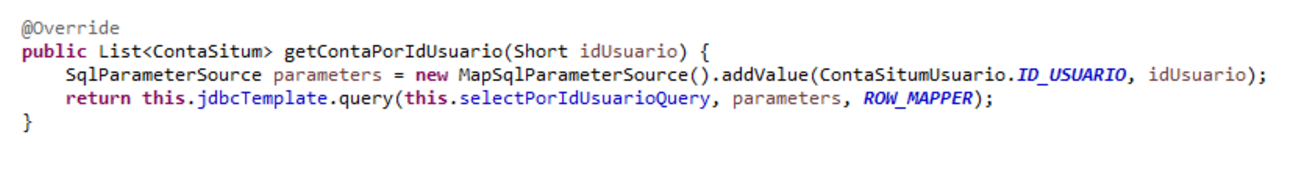
\includegraphics[width=1\textwidth]{figures/codigo/daoConsulta}
		\caption{Método de consulta dun DAO.}
		\label{fig:daoConsulta}
	\end{center}
\end{figure}

As consultas a base de datos lánzanse a través de \emph{jdbcTemplate}, como se pode observar na figura~\ref{fig:daoConsulta}. Neste exemplo lánzase a consulta inxectada no atributo \emph{selectPorIdUsuarioQuery} cos parámetros que se engaden previamente, que é o identificador do usuario. Os datos gárdanse no VO grazas ao mapa definido en \emph{ROW\_MAPPER}, que se pode ver na figura~\ref{fig:daoRowMapper}.

\begin{figure}[tbh] 
	\begin{center}
		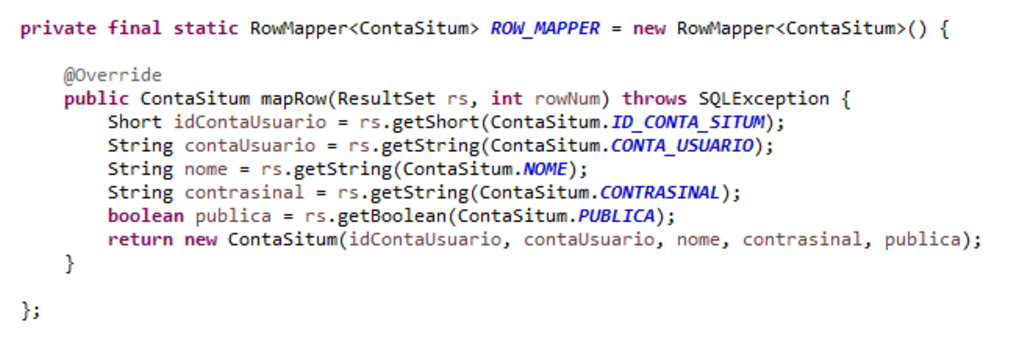
\includegraphics[width=0.9\textwidth]{figures/codigo/daoRowMapper}
		\caption{Construción dun VO dentro do DAO.}
		\label{fig:daoRowMapper}
	\end{center}
\end{figure}

En canto á consulta mencionada no parágrafo anterior, podemos ver como está no ficheiro de consultas na figura~\ref{fig:daoConsultaSQL}. Pódese apreciar a maneira de marcar o lugar onde se situarían os parámetros introducidos no método do DAO, :ID\_USUARIO, neste caso. Cando se executa a consulta substitúese esa cadea de texto polo valor inserido no método como se viu na figura~\ref{fig:daoConsulta}.

\begin{figure}[tbh] 
	\begin{center}
		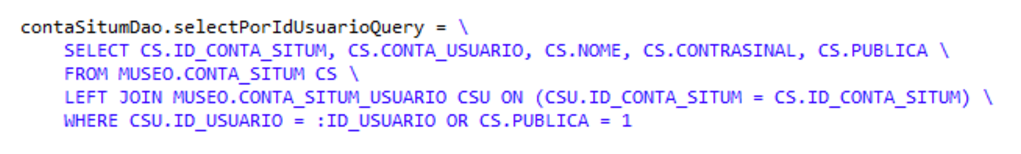
\includegraphics[width=0.8\textwidth]{figures/codigo/daoConsultaSQL}
		\caption{Exemplo dunha consulta en SQL.}
		\label{fig:daoConsultaSQL}
	\end{center}
\end{figure}

Por último, amosar como se levaría a cabo unha sentencia de inserción ou modificación de datos dentro dos DAOs. Na figura~\ref{fig:daoInsert} pódese ver como se establecen os valores para a inserción dunha nova conta de Situm dentro da base de datos e como se utiliza o método \emph{update} pasándolle a sentencia e o mapa cos parámetros.

\begin{figure}[tbh] 
	\begin{center}
		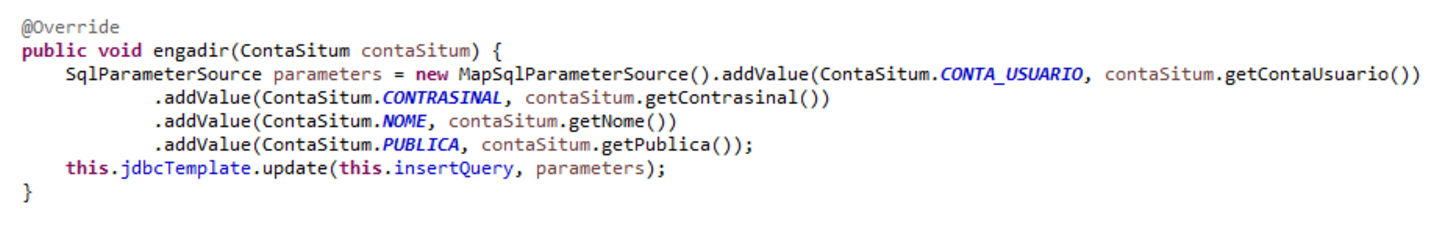
\includegraphics[width=1\textwidth]{figures/codigo/daoInsert}
		\caption{Método de inserción dun DAO.}
		\label{fig:daoInsert}
	\end{center}
\end{figure}


\subsection{Transaccionalidade}
A xestión transaccionalidade impleméntase na capa Manager utilizando o framework Spring, grazas á súa librería spring-tx. A súa configuración e utilización é moi sinxela, tal e como se pode observar nos exemplos. No primeiro amósase a configuración que require nos ficheiros XML de Spring. Para indicar a transaccionalidade, utilizaremos etiquetas que permitan identificar o tipo de transacción que queremos que se aplique en cada método público do manager. Non todos os métodos provocan escrituras en base de datos, polo que non será necesario indicar o tipo de transaccionalidade que provoca desfacer cambios en todos eles. O resto marcaranse como de só lectura para non sobrecargar innecesariamente o sistema.

Na figura~\ref{fig:transaccionConfiguracion} pódese observar a configuración da transaccionalidade nos ficheiros XML.

\begin{figure}[tbh] 
	\begin{center}
		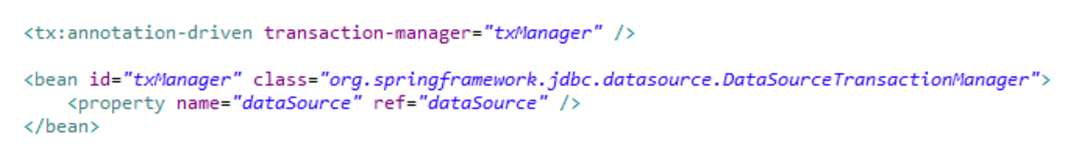
\includegraphics[width=1\textwidth]{figures/codigo/transaccionConfiguracion}
		\caption{Configuración da transaccionalidade no ficheiro XML.}
		\label{fig:transaccionConfiguracion}
	\end{center}
\end{figure}


Na figura~\ref{fig:metodoTransaccional} pódese observar a configuración da transaccionalidade sobre un método no que se modifican datos.

\begin{figure}[tbh] 
	\begin{center}
		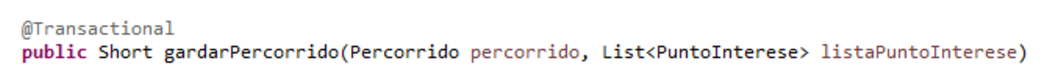
\includegraphics[width=1\textwidth]{figures/codigo/metodoTransaccional}
		\caption{Configuración da transaccionalidade dun método onde se modifican datos.}
		\label{fig:metodoTransaccional}
	\end{center}
\end{figure}

Na figura~\ref{fig:metodoNonTransaccional} pódese observar a configuración da transaccionalidade sobre un método de só lectura.

\begin{figure}[tbh] 
	\begin{center}
		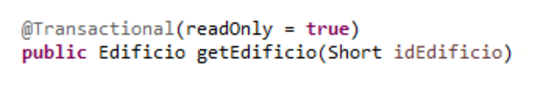
\includegraphics[width=0.5\textwidth]{figures/codigo/metodoNonTransaccional}
		\caption{Configuración da transaccionalidade dun método de só lectura.}
		\label{fig:metodoNonTransaccional}
	\end{center}
\end{figure}


\subsection{Construción dos servizos web}
Para a construción dos servizos web creáronse dous controladores distintos, tal e como se comentou na sección de deseño: un para as imaxes e o outro para o resto de información. Esta capa comunícase coa capa dos manager, detallada na subsección anterior. Para a súa implementación usouse unha librería específica de Spring para a construción de servizos web: Spring MVC.

\begin{figure}[tbh] 
	\begin{center}
		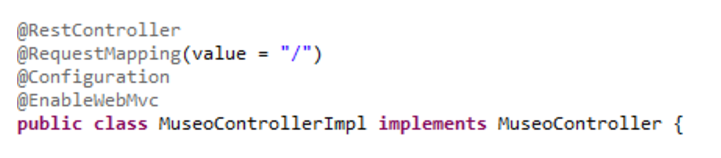
\includegraphics[width=0.7\textwidth]{figures/codigo/controladorMuseo}
		\caption{Exemplo de etiquetas sobre o servizo.}
		\label{fig:controladorMuseo}
	\end{center}
\end{figure}

Na figura~\ref{fig:controladorMuseo} pódese observar como se configura un controlador do servizo. Coa etiqueta \emph{@RestController} identifícanse as clases que actúan como controladores de servizos web REST, ao mesmo tempo que indica que o valor de retorno dos métodos vai no corpo da response. Dentro destas clases inclúense os métodos que estarán publicados no servizo coas súas propias anotacións. A continuación veranse distintos exemplos dos tipos de métodos que se publican no noso servizo.

\begin{figure}[tbh] 
	\begin{center}
		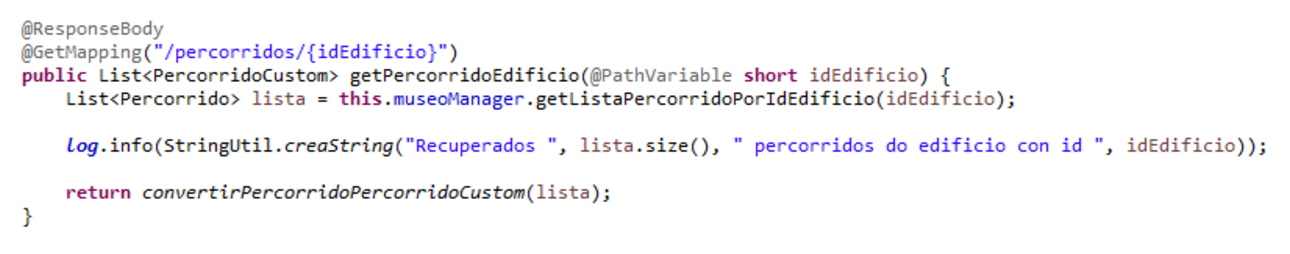
\includegraphics[width=0.7\textwidth]{figures/codigo/chamadaServizoGetParametro}
		\caption{Exemplo de método Get con parámetro do servizo.}
		\label{fig:chamadaServizoGetParametro}
	\end{center}
\end{figure}

O primeiro método a observar é de tipo GET, é dicir, de recuperación de información. No caso da figura~\ref{fig:chamadaServizoGetParametro} tense unha etiqueta \emph{@GetMapping} coa que se indica o seu tipo e a continuación a URL que activa ese método. Nas chamadas REST pódense introducir variábeis na propia URL, como ocorre neste caso co parámetro \emph{idEdificio}. Para poder utilizar esta variábel débese indicar como parámetro dentro do método e anotala coa etiqueta \emph{@PathVariable} e nomeala do mesmo xeito.

\begin{figure}[tbh] 
	\begin{center}
		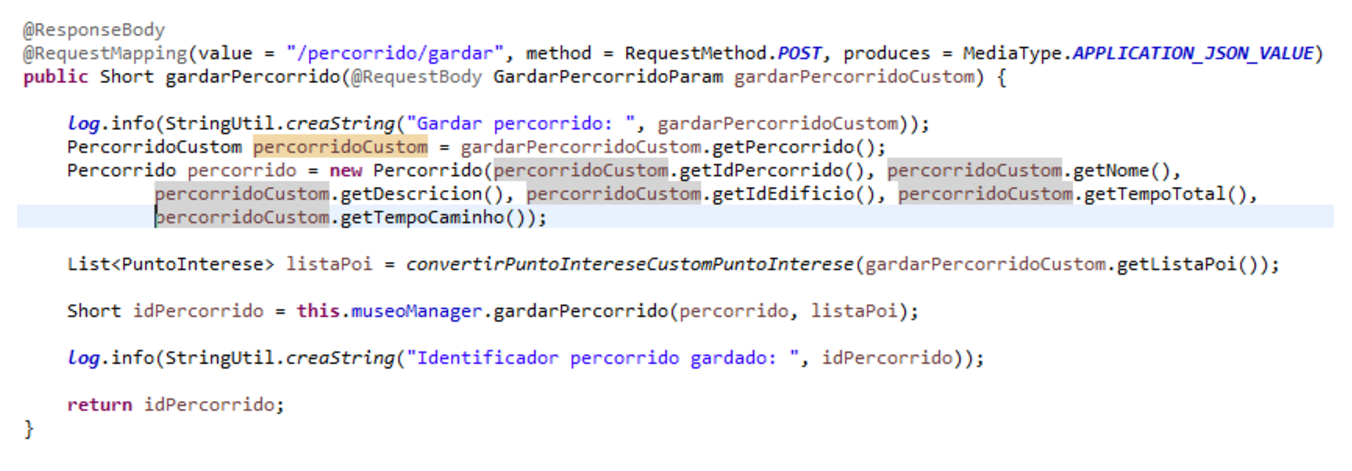
\includegraphics[width=1\textwidth]{figures/codigo/chamadaServizoPost}
		\caption{Exemplo de método Post do servizo.}
		\label{fig:chamadaServizoPost}
	\end{center}
\end{figure}

Outro tipo de métodos dentro do noso servizo web é o POST, utilizado para enviar información ao servidor e realizar modificacións. Na figura~\ref{fig:chamadaServizoPost} obsérvase un exemplo deste tipo. Pasar parámetros a través da URL non é a única maneira de enviar datos a un servizo REST, xa que se pode utilizar o corpo da request coma neste caso. Spring MVC interpreta o corpo da request coma un JSON e tradúceo a un obxecto do servidor automaticamente xa que está construído cos mesmos atributos. Para indicar que o parámetro provén do corpo da request utilízase a etiqueta \emph{@RequestBody}.

\begin{figure}[tbh] 
	\begin{center}
		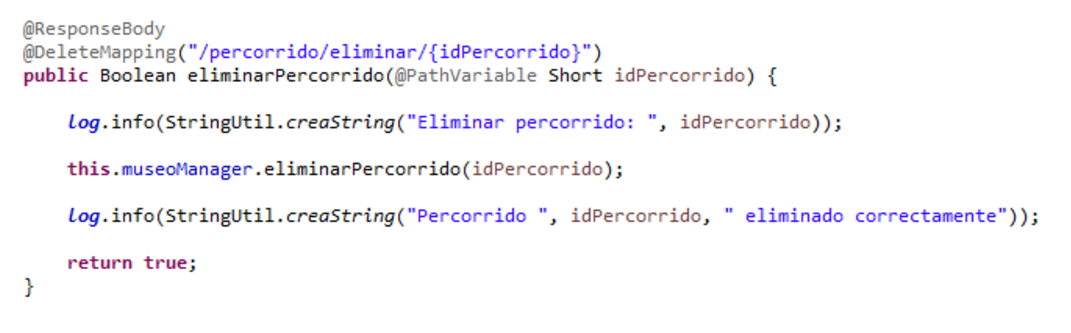
\includegraphics[width=0.7\textwidth]{figures/codigo/chamadaServizoDelete}
		\caption{Exemplo de método Delete do servizo.}
		\label{fig:chamadaServizoDelete}
	\end{center}
\end{figure}

Por último, quedan os métodos DELETE, utilizados para eliminar información do servidor. Na figura~\ref{fig:chamadaServizoDelete} pode observarse un método deste tipo utilizado no noso servizo. Nel pode verse como recibe un parámetro pola URL e como devolve un boolean no corpo da response indicando se houbo éxito no borrado do punto de interese.


\subsection{Autorización nos servizos}
Tal e como se indicou no apartado de deseño de "Securización das comunicacións", implementouse un sistema de autenticación básica sobre os servizos web, de tal maneira que non se permite a chamada a eses servizos se non se inclúe na cabeceira un token para a autenticación. Este token constrúese mediante a codificación en Base64 dun nome de usuario e contrasinal que son comúns ás chamadas. A configuración desta securización realízase no ficheiro web.xml, onde se inclúe o código da figura~\ref{fig:configuracionAutenticacion}.

\begin{figure}[htb] 
	\begin{center}
		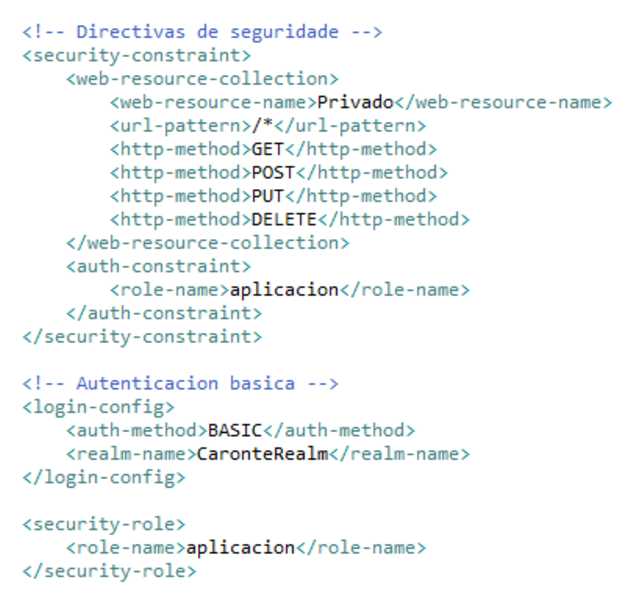
\includegraphics[width=0.6\textwidth]{figures/codigo/configuracionAutenticacion}
		\caption{Configuración da autenticación básica no servidor.}
		\label{fig:configuracionAutenticacion}
	\end{center}
\end{figure}

Como se pode observar na figura, securízanse as chamadas GET, DELETE, POST e PUT, que son as básicas nos servizos REST. Calquera chamada que non teña o token de autenticación correcto será rexeitada sen entrar no servizo.


\section{Aplicación Android}
Nesta sección trataranse os aspectos máis importantes da implementación na aplicación Android.

\subsection{Solicitude de permisos}
A aplicación Android require de certos permisos para o seu correcto funcionamento. Actualmente non é preciso aceptar o uso destes permisos na propia instalación do APK, senón que se permite a solicitude individual dentro da aplicación, cando se precisan por primeira vez. Os permisos solicitados pola aplicación débense indicar no AndroidManifest.xml e pódense ver na figura~\ref{fig:permisos}.

\begin{figure}[htb] 
	\begin{center}
		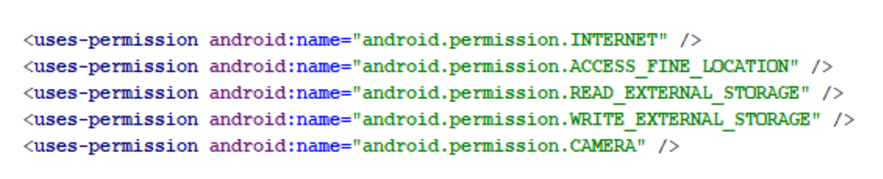
\includegraphics[width=0.6\textwidth]{figures/codigo/permisos}
		\caption{Permisos necesarios na aplicación Android.}
		\label{fig:permisos}
	\end{center}
\end{figure}

Non faría falla indicar a solicitude do permiso para o acceso a internet nas versións actuais de Android, mais indícase para os dispositivos que utilicen versións antigas. Deixou de ser preciso aceptar este permiso debido a que a inmensa maioría de aplicacións fan uso de internet.

\begin{figure}[htb] 
	\begin{center}
		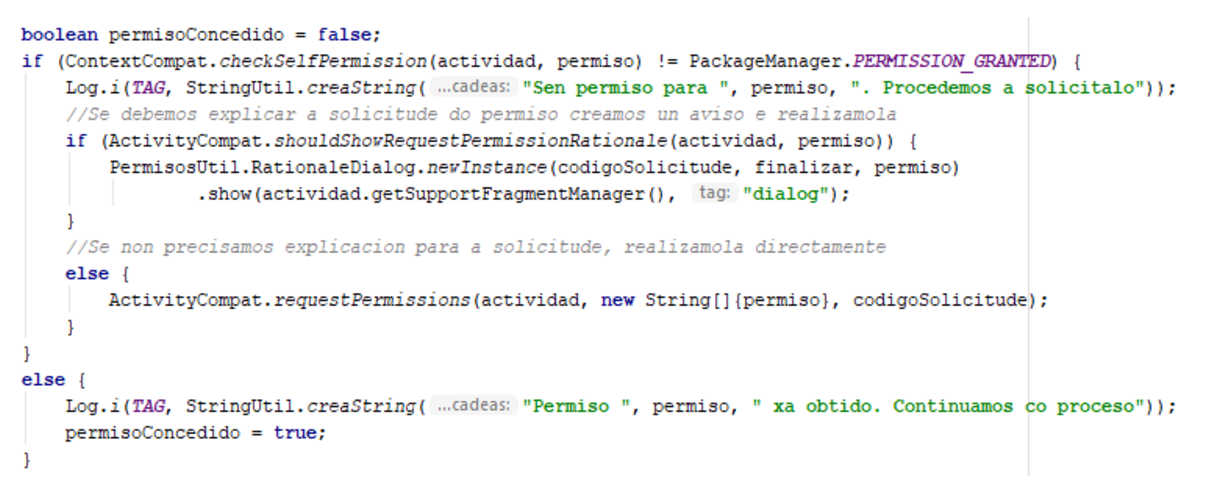
\includegraphics[width=1\textwidth]{figures/codigo/solicitudePermisos}
		\caption{Comprobación e solicitude de permisos necesarios na aplicación Android.}
		\label{fig:solicitudePermisos}
	\end{center}
\end{figure}

Antes da realización de calquera acción que requira permisos especiais é obrigatorio comprobar se a aplicación ten acceso a ese permiso, xa que o usuario pode revocalo en calquera momento. No caso de que non o teña, aparecerá un diálogo na pantalla que pregunte ao usuario se desexa permitir esa acción. Se acepta, continuará a execución sen problema, se non o acepta e o permiso era imprescindíbel, a aplicación deixará de funcionar. A comprobación e solicitude dos permisos realízanse mediante chamadas específicas proporcionadas polas propias librerías de Android, polo que apenas require esforzo por parte do programador. Un exemplo de código pódese ver na figura~\ref{fig:solicitudePermisos}.

\todo{https://developer.android.com/training/permissions/requesting?hl=es-419}

\subsection{Acceso a Situm}
Neste punto revisarase a configuración dos servizos de Situm e por outra parte, a solicitude de información sobre os edificios.

\subsubsection{Configuración da localización}
O primeiro paso para configurar o acceso a Situm é engadir a dependencia coa súa librería tal e como se indicou na sección de deseño. Unha vez se ten esa dependencia, pódese facer uso de certas clases e métodos para poder acceder aos servizos de Situm.

\begin{figure}[htb] 
	\begin{center}
		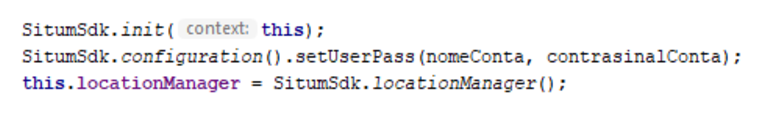
\includegraphics[width=0.7\textwidth]{figures/codigo/situmInicio}
		\caption{Inicialización do SDK de Situm.}
		\label{fig:situmInicio}
	\end{center}
\end{figure}

Para inicializar o SDK de Situm débese realizar unha chamada específica dentro do código e posteriormente indicar o usuario e o contrasinal co cal se quere acceder aos servizos. Estas accións pódense ver na figura~\ref{fig:situmInicio}.

\begin{figure}[htb] 
	\begin{center}
		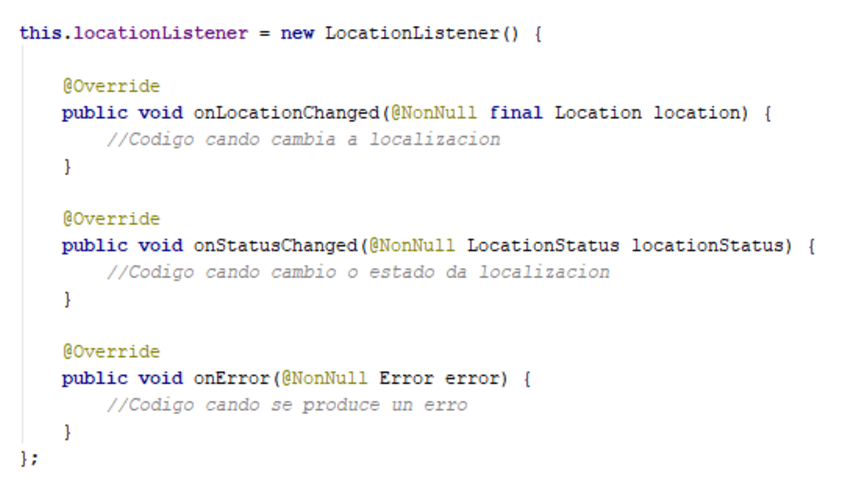
\includegraphics[width=0.7\textwidth]{figures/codigo/situmLocationManager}
		\caption{Creación do location manager de Situm.}
		\label{fig:situmLocationManager}
	\end{center}
\end{figure}

Unha vez inicializado, o seguinte paso sería a activación da localización en interiores. Para realizar isto débese solicitar esta activación aos servidores de Situm, mais antes de realizar este paso débese comprobar se a aplicación dispón do permiso de localización, imprescindíbel para o uso da aplicación. Mediante a creación dun listener específico permítese a resposta á información devolta por parte de Situm no referente á posición. Este listener (na figura~\ref{fig:situmPosicionamento}) dispón de tres métodos para reaccionar ante cambios de posición, cambios de estado ou erros no servizo. O método principal ao que máis importancia lle debemos dar é ao de cambio de posición, xa que é o que máis vai modificar o estado da nosa aplicación. Devolve a información da posición actual do usuario: edificio, piso, coordenadas, orientación, entre outras. O segundo método informa sobre o estado actual do sistema, ben se está inicializado, en proceso de arranque, se o usuario non se atopa nun edificio, etcétera. Por último tense o método que recibe os erros de Situm que provoquen a detención do posicionamento.

\begin{figure}[htb] 
	\begin{center}
		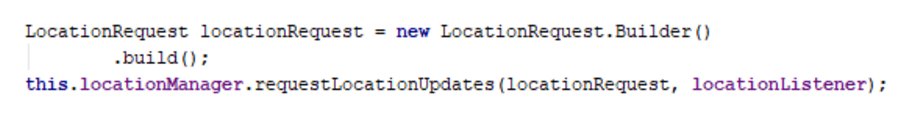
\includegraphics[width=0.8\textwidth]{figures/codigo/situmPosicionamento}
		\caption{Activación do posicionamento de Situm.}
		\label{fig:situmPosicionamento}
	\end{center}
\end{figure}

Cando se dispoña do listener, pódese iniciar o posicionamento mediante o código amosado na figura~\ref{fig:situmPosicionamento}. A partir dese momento comezarán a chegar notificacións no listener definido no punto anterior.

\subsubsection{Acceso aos servizos de Situm}
Aínda que a maioría dos datos dos que ten que facer uso a aplicación proveñen do noso propio servidor, tamén se debe recuperar certa información dos servidores de Situm. As chamadas que se deben realizar aos servidores de Situm son as seguintes:

\begin{itemize}
	\item Recuperación da lista cos edificios aos que ten acceso esa conta (nada máis establecer a conta de Situm).
	\item Recuperación da lista dos niveis dun edificio concreto (cando se accede a ese edificio).
	\item Recuperación dos mapas dos niveis dun edificio que se amosarán enriba do fragmento de Google Maps.
	\item Recuperación da ruta a un punto concreto do mapa. Se as rutas están configuradas en Situm e nos atopamos fisicamente dentro dun edificio, a aplicación permite solicitar rutas para dirixirse ao punto desexado, amosando as direccións que debe seguir o usuario.
\end{itemize}

\begin{figure}[htb] 
	\begin{center}
		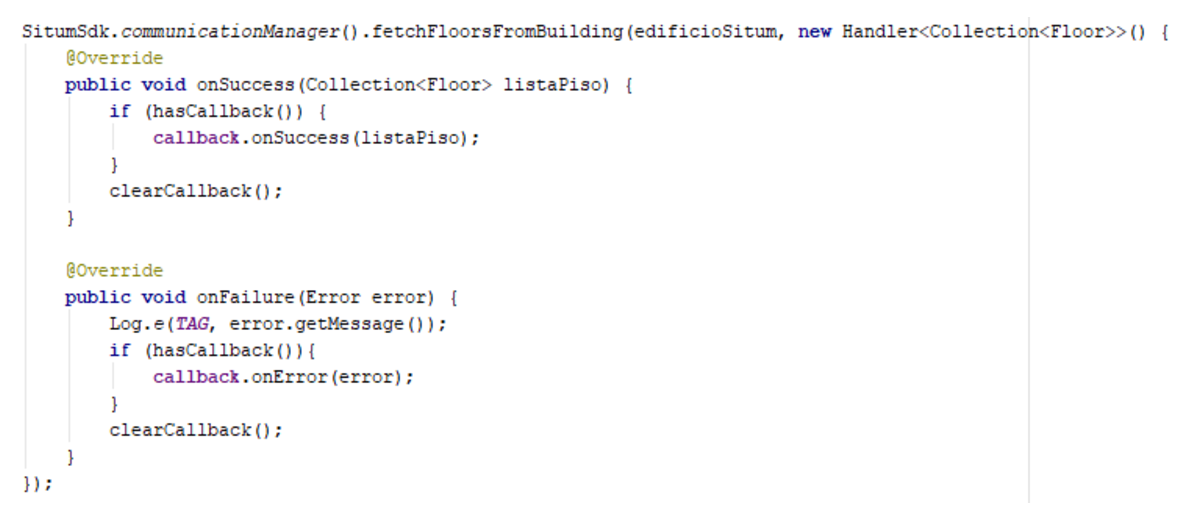
\includegraphics[width=0.9\textwidth]{figures/codigo/situmExemploChamada}
		\caption{Chamada para a recuperación dos niveis dun edificio en Situm.}
		\label{fig:situmExemploChamada}
	\end{center}
\end{figure}

Para o acceso aos servizos de Situm optouse por illar as conexións en clases distintas para identificar mellor a lóxica levada a cabo en cada unha delas. Estas clases atópanse no paquete gal.caronte.servizo.situm. Os accesos aos servidores de Situm realizáronse mediante o uso da SDK de Situm na súa versión 2.9.0.

A conexión realízase mediante o Communication Manager de Situm, un xestor que se obtén mediante unha chamada específica. Unha vez se ten ese xestor, pódese solicitar a información desexada aos servidores de Situm mediante os métodos que dispón. Un exemplo destas chamadas pode verse na figura~\ref{fig:situmExemploChamada}, onde se recuperan os niveis dun edificio concreto.


\subsection{Acceso ao servidor}
Ao igual que se explicou no punto anterior para as conexións con Situm, as conexións co servidor propio da aplicación tamén se realizaron en clases illadas para non mesturar o código de diversas solicitudes. As chamadas son asíncronas polo que se poden realizar varias á vez e continuar coa execución da aplicación normalmente.

As chamadas ao servidor propio son distintas na súa realización. Débese indicar a dirección e incluír os datos de autorización na cabeceira en cada unha delas. Non é a única información que se deber proporcionar ao lanzar esas solicitudes, senón que tamén se ten que indicar en que formato converter os datos (JSON) e en que tipo de dato converter a resposta.

\begin{figure}[htb] 
	\begin{center}
		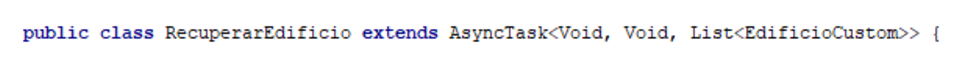
\includegraphics[width=0.8\textwidth]{figures/codigo/chamadaServidorDefinicion}
		\caption{Construción dunha clase de acceso ao servidor de Caronte.}
		\label{fig:chamadaServidorDefinicion}
	\end{center}
\end{figure}

Na figura~\ref{fig:chamadaServidorDefinicion} pódese ver o formato das clases utilizadas para a comunicación co servidor. Deben estender a clase \emph{AsyncTask} e indicar os tipos dos datos enviados ao servidor (primeiro dos xenéricos) e os datos que se recibirán (terceiro dos xenéricos). Neste exemplo non se envían parámetros na chamada e se recibe unha lista de edificios, que se verán nas seguintes figuras.

\begin{figure}[htb] 
	\begin{center}
		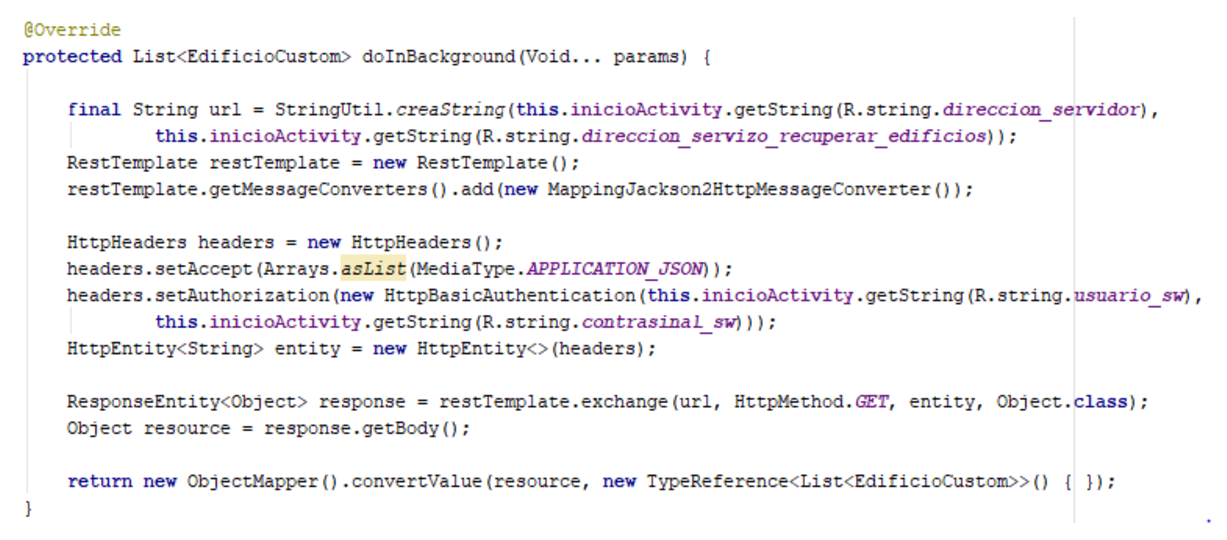
\includegraphics[width=1\textwidth]{figures/codigo/chamadaServidorBackground}
		\caption{Método para a realización dunha chamada ao servidor de Caronte.}
		\label{fig:chamadaServidorBackground}
	\end{center}
\end{figure}

O método dende o cal se realiza a chamada pódese observar na figura~\ref{fig:chamadaServidorBackground}. O primeiro punto a ter en conta é o tipo dos parámetros que recibe o método: Void; iso indica que este método non recibe ningún parámetro para enviar ao servidor mais si se pode ver que ten un tipo de retorno, unha lista de edificios que se tratarán despois. Pode apreciarse a construción da URL á que se vai realizar a chamada, o convertedor da mensaxe ao formato desexado (JSON), a cabeceira onde se indica o formato e os datos para a autorización básica da chamada.

As últimas sentencias do método son a propia chamada ao servidor onde se indica a URL, o tipo de chamada (GET), as entidades da solicitude (neste caso só a cabeceira) e o tipo de dato que devolve o método. A continuación poderíanse indicar os parámetros que se queren enviar coa petición separados por comas, pero nesta chamada non hai ningún. Como esta chamada tarda tempo en devolver os datos desexados semella que o fluxo queda detido neste punto, mais como xa se indicou antes, a chamada é asíncrona e pode continuar a execución da aplicación con normalidade. O último paso sería converter os datos recibidos ao tipo de obxecto desexado.


\begin{figure}[htb] 
	\begin{center}
		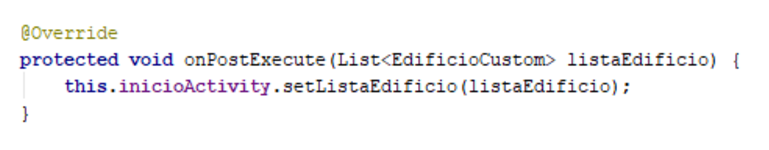
\includegraphics[width=0.7\textwidth]{figures/codigo/chamadaServidorPost}
		\caption{Método para o tratamento de datos devoltos por unha chamada ao servidor de Caronte.}
		\label{fig:chamadaServidorPost}
	\end{center}
\end{figure}


Para poder facer uso dos datos recibidos, existe outro método nestas clases de acceso ao servidor, e é o método \emph{onPostExecute}, que recibe como parámetro o tipo de dato devolto no método \emph{doInBackground}. Cando remata a execución da chamada os datos acabarán chegando a este método dende onde se poderán realizar as accións desexadas con eles.


\section{Autenticación}
Neste punto verase o proceso de autenticación en máis profundidade, revisando as diferentes chamadas necesarias tanto dende a aplicacion Android coma dende o servidor contra os servizos de Google para verificar a identidade do usuario.

O primeiro punto a ter en conta é a configuración necesaria para permitir a autenticación dende a aplicación. Débese incluír a dependencia con \emph{'com.google.android.gms:play-services-auth:12.0.1'} no build.gradle a nivel de aplicación e incluír o ficheiro google-services.json específico de Caronte que se pode conseguir despois de dar de alta o proxecto na consola de desenvolvemento de Google. Dende esta mesma consola pódense conseguir as credenciais que permiten a conexión cos servizos de Google que utilizaremos a continuación, na conexión dende a aplicación Android e dende o servidor.


\todo{https://console.developers.google.com/apis/credentials}

\todo{incluir referencia a https://developers.google.com/identity/sign-in/android/start-integrating}

\todo{https://developers.google.com/android/guides/client-auth}

\begin{figure}[htb] 
	\begin{center}
		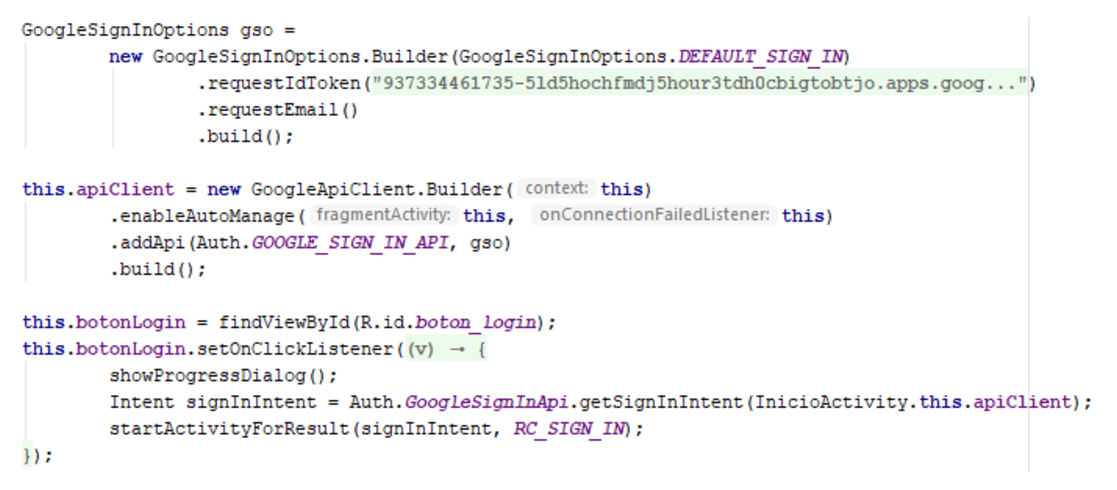
\includegraphics[width=0.9\textwidth]{figures/codigo/autenticacionGoogleInicio}
		\caption{Código para a autenticación con Google na aplicación.}
		\label{fig:autenticacionGoogleInicio}
	\end{center}
\end{figure}

O primeiro paso para permitir o acceso a un usuario concreto na aplicación é a obtención das credenciais de autenticación do usuario. Para lograr isto, temos o código da figura~\ref{fig:autenticacionGoogleInicio}. Pulsando sobre o botón de login lanzarase unha actividade propia de Google que permite a autenticación dentro da aplicación cunha conta de Google.

\begin{figure}[htb] 
	\begin{center}
		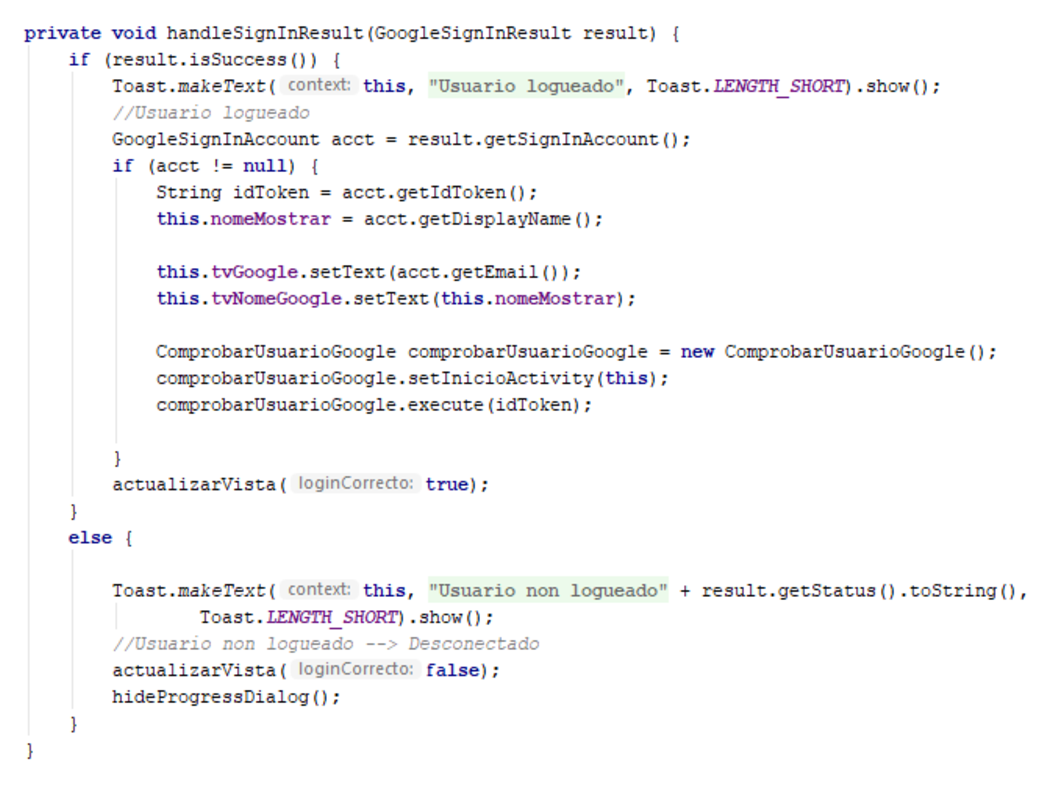
\includegraphics[width=0.9\textwidth]{figures/codigo/autenticacionGoogleRecepcion}
		\caption{Código para a autenticación con Google na aplicación (2).}
		\label{fig:autenticacionGoogleRecepcion}
	\end{center}
\end{figure}

O seguinte paso será o tratamento da información recibida cando a actividade lanzada no punto anterior remate correctamente. Pódese ver na figura~\ref{fig:autenticacionGoogleRecepcion} o tratamento dos datos. O punto principal é o lanzamento dunha chamada ao servidor de Caronte pasando como parametro un token enviado por Google para verificar a conta.

\begin{figure}[htb] 
	\begin{center}
		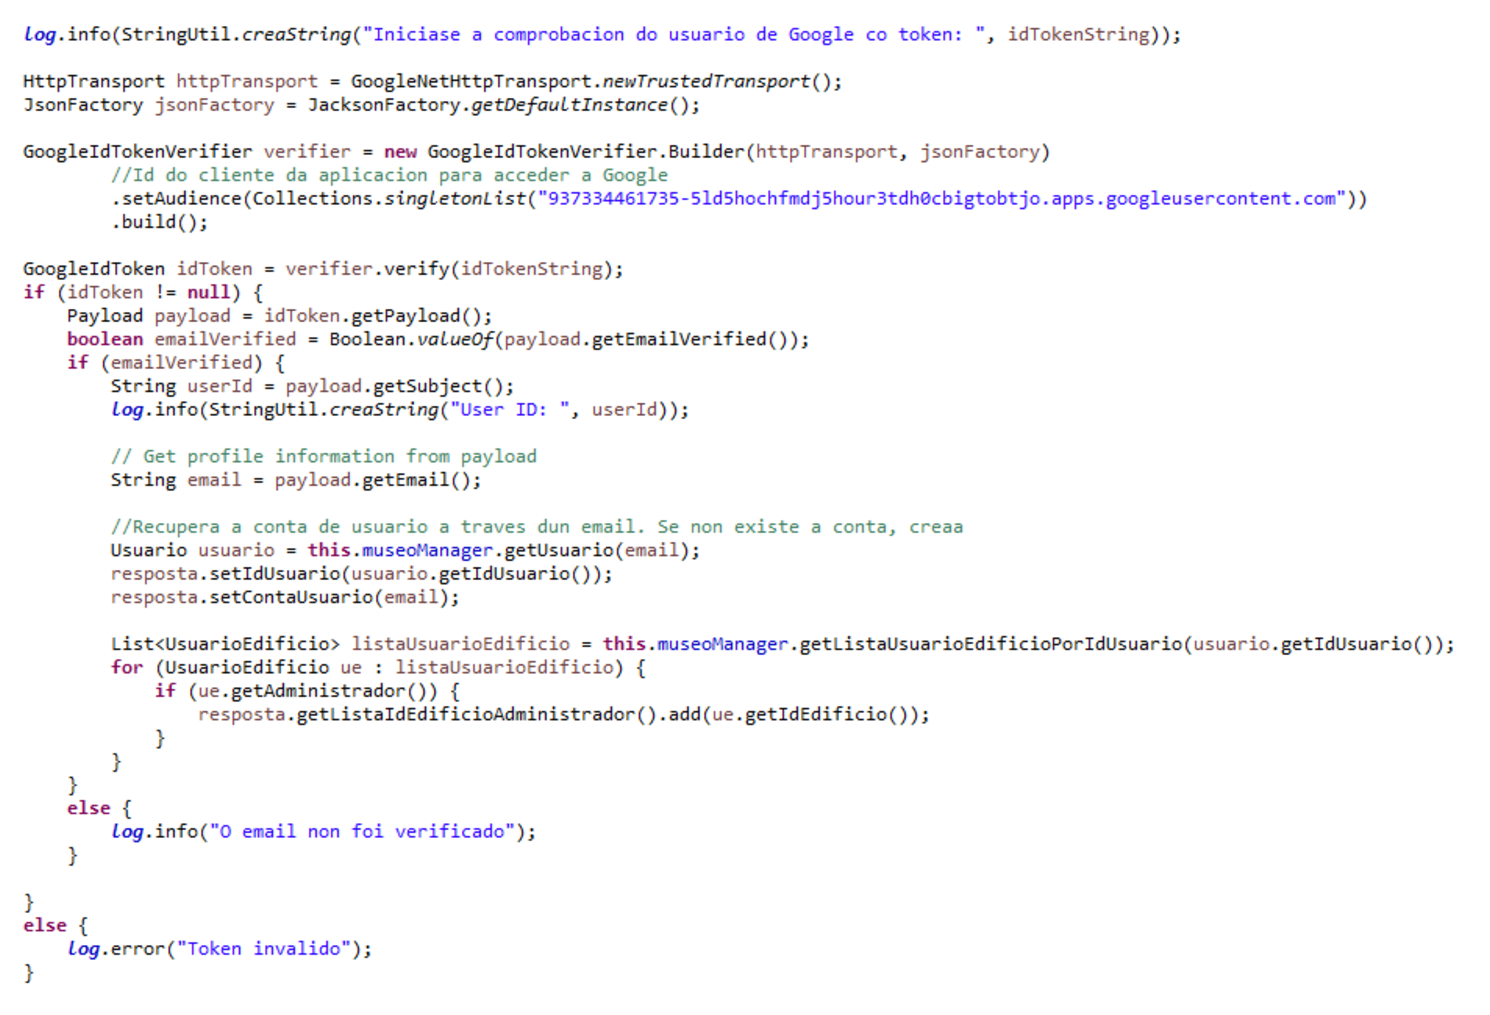
\includegraphics[width=1\textwidth]{figures/codigo/autenticacionGoogleServidor}
		\caption{Código para a autenticación con Google na aplicación (e 3).}
		\label{fig:autenticacionGoogleServidor}
	\end{center}
\end{figure}

Na figura~\ref{fig:autenticacionGoogleServidor} pódese ver o código do servidor co cal se verifica a conta coa que se acaba de autenticar o usuario. Utilízase a clase GoogleIdTokenVerifier para verificar o token recibido na aplicación Android. Se o token é válido, devólvese a información do usuario xunto cos seus roles á aplicación Android, se ten algún. Se é a primeira vez que o usuario accede ao sistema, gardarase a súa conta na base de datos.

Para que funcione a autenticación desde unha aplicación descargada de Google Play débese incluír a chave do certificado co que se firma a aplicación na consola para desenvolvedores de Google.

\todo{Para publicar a aplicación na Play Store}
\todo{https://developer.android.com/studio/publish/app-signing}
